% IEEE BigData 2026 Regular Paper (conference 2-column, up to 10 pages incl. references)
\documentclass[conference]{IEEEtran}
\IEEEoverridecommandlockouts
\usepackage{cite}
\usepackage{amsmath,amssymb,amsfonts,amsthm}
\usepackage{graphicx}
\usepackage{textcomp}
\usepackage{xcolor}
\usepackage{booktabs}
\usepackage{array}
\usepackage{multirow}
\usepackage{tabularx}
\usepackage{tikz}
\usepackage{siunitx}
\usepackage{bbm}
\usepackage{placeins}
\usepackage{balance}
\usepackage{url}
\usetikzlibrary{shapes.geometric, arrows.meta, positioning, fit, backgrounds}
\def\BibTeX{{\rm B\kern-.05em{\sc i\kern-.025em b}\kern-.08em
    T\kern-.1667em\lower.7ex\hbox{E}\kern-.125emX}}

\graphicspath{{./}{../}{figures/}{../figures/}{paper_visuals/}{./paper_visuals/}}

\newtheorem{theorem}{Theorem}
\newtheorem{remark}{Remark}
\newtheorem{definition}{Definition}
\newtheorem{proposition}{Proposition}

\raggedbottom
\renewcommand{\topfraction}{0.95}
\renewcommand{\bottomfraction}{0.90}
\renewcommand{\textfraction}{0.05}
\renewcommand{\floatpagefraction}{0.75}
\setcounter{topnumber}{3}
\setcounter{bottomnumber}{2}
\setcounter{totalnumber}{5}

\begin{document}

\title{HARP: Hop-Aware Selective Release\\
for Privacy-Audited GNN Prediction APIs}

\author{\IEEEauthorblockN{Krish Sharma}
\IEEEauthorblockA{\textit{Academy of Math, Science, and Applied Technology}\\
\textit{Ed W. Clark High School}\\
Las Vegas, NV, USA\\
krish.sharma@unlv.edu\\
\thanks{Research conducted with the Data Science Laboratory (DiSC), University of Nevada, Las Vegas.}}
\and
\IEEEauthorblockN{Shaikh Arifuzzaman}
\IEEEauthorblockA{\textit{Department of Computer Science}\\
\textit{University of Nevada, Las Vegas}\\
Las Vegas, NV, USA\\
shaikh.arifuzzaman@unlv.edu}
}

\maketitle

\begin{abstract}
Graph neural networks are increasingly served as prediction APIs: clients query a node and receive a softmax score vector used for ranking, routing, and analytics on graphs from thousands to millions of nodes.
At this scale the API is a continuous data product---operators must keep accuracy high, keep most responses bit-exact for caching and compliance, and remain \emph{audit-compliant} under membership inference checks.
Uniform Laplace posterior perturbation (LBP) cannot meet that joint goal: any $b{>}0$ perturbs \emph{every} response, so a clean-majority constraint is infeasible by construction.
We formalize this as \emph{constrained score release}---maximize accuracy subject to a membership audit and a minimum exact-response fraction---and propose \textbf{HARP}, a selective release framework for GNN score APIs.
\textbf{HARP is not proposed as a stronger membership defense than uniform noise}; it is the mechanism that can satisfy a clean-majority constraint while remaining audit-compliant and recovering accuracy versus published strong LBP.
HARP ranks nodes (topology or audit-guided vulnerability), expands high-risk seeds by $k$ hops, and applies a protector only on that set, with Frac/Mass dials and a session budget against re-query averaging.
Across six graphs, GAT/inductive checks, ogbn-arxiv (${\sim}169$k) with defense-aware LiRA, and an ogbn-products subsampled audit (${\sim}15$k of $2.4$M), HARP recovers large accuracy drops versus strong LBP while enabling a $60\%$ clean majority that uniform noise cannot provide.
\end{abstract}

\begin{IEEEkeywords}
graph neural networks, prediction APIs, Big Data systems, selective release, data quality, membership inference
\end{IEEEkeywords}

\section{Introduction}

\subsection{Motivation}
Graph neural networks (GNNs) are widely deployed as \emph{prediction APIs}: a client queries a node ID and receives a softmax score vector~\cite{kipf2017gcn,hamilton2017graphsage}.
Those scores drive ranking, triage, and analytics.
They also leak whether a node was in the training set, via membership inference attacks (MIAs)~\cite{shokri2017membership,salem2019mlleaks,carlini2022membership,olatunji2021mia}.

At Big Data scale the API is not a one-shot model export.
It is a stream of released probabilities.
Operators therefore face three systems concerns:
\textbf{volume} (graphs from $10^3$ to $10^6+$ nodes),
\textbf{velocity} (clients may re-query randomized answers),
and \textbf{veracity} (many pipelines need stable, well-calibrated scores for caching, A/B tests, and compliance).

The usual graph defense is Laplace posterior perturbation (LBP)~\cite{olatunji2021mia}.
Strong uniform noise ($b{=}0.3$) lowers attack success but often collapses accuracy.
Weaker noise keeps accuracy but still perturbs \emph{every} node and raises expected calibration error (ECE).
Neither option yields a \emph{clean majority} of exact scores---a concrete data-quality property for downstream consumers.

The systems question is therefore \textbf{constrained budget allocation}: maximize task accuracy subject to a membership audit \emph{and} a minimum fraction of bit-exact responses.

\paragraph{Main idea.}
Membership signal on graphs is not node-local: message passing mixes neighborhoods.
HARP (Hop-Aware selective Release Policy) ranks nodes with a cheap topology estimator (LTE) or an audit-guided vulnerability score, expands high-risk seeds by $k$ hops into a protected set $\mathcal{P}_k$, and applies a protector (strong Laplace or selective masking) \emph{only} on that set.
Under our locked setting (protected fraction Frac${=}0.40$), about $60\%$ of API responses stay bit-exact---impossible for any uniform $b{>}0$.

\subsection{Gap}
Prior defenses include LBP~\cite{olatunji2021mia}, MemGuard~\cite{jia2019memguard}, train-time GNN MIA methods (GTD, MaskArmor)~\cite{gtd2024,maskarmor2024}, AdvReg~\cite{nasr2018advreg}, and training-time DP-GNNs~\cite{sajadmanesh2023gap,napgnn2023,abadi2016deepdp,dwork2006dp}.
MemGuard and uniform LBP both perturb every response; train-time methods do not expose Mass/Frac release accounting.
None treat ExactFrac$\ge c{>}0$ as a hard systems constraint on a hop-coupled GNN API, nor expose constructor$\times$protector dials under matched-budget audits.
HARP targets that systems gap---reusing known protectors inside a new allocation problem.

\paragraph{Running example.}
On Cora ($n{=}2708$), strong LBP cuts accuracy from ${\approx}0.88$ to ${\approx}0.71$.
Weak uniform noise preserves accuracy but perturbs every score (ECE ${\approx}0.16$).
HARP matches that weak-noise budget, keeps ${\approx}60\%$ of scores exact, reaches ECE ${\approx}0.033$ and Acc ${\approx}0.83$, and only modestly changes membership-attack AUROC.
The operator gains usable accuracy and reproducible scores for most queries---not a claim that clean nodes are ``membership-safe.''

\paragraph{Non-goal (stated up front).}
HARP is \emph{not} a claim of lower population LiRA than equal-mass or strong uniform LBP.
When ExactFrac$=0$ is allowed, uniform noise is often the better Acc--LiRA point.
HARP's claim is narrower and systems-shaped: it is the feasible class of policies under ExactFrac$\ge c{>}0$, with hop-consistent allocation, operator dials, and Acc/calibration recovery versus the published strong-LBP recipe.

\paragraph{Novelty (what is new).}
The conceptual contribution is the \emph{problem}, not a new noise distribution.
Prior release defenses answer ``how to perturb a score''; HARP answers ``how to allocate a release budget on a message-passing API when a clean majority is mandatory.''
Laplace and masking are interchangeable \emph{protectors}---pluggable baselines, not the invention.
What is new is constrained score release with ExactFrac as a first-class constraint, hop-consistent protected-set geometry, and Mass/Frac/\(B\) telemetry under matched-budget audits.

\subsection{Contributions and paper map}
\begin{enumerate}
  \item \textbf{Constrained score release.} Formalize maximize Acc s.t.\ LiRA$\le\tau$ and ExactFrac$\ge c$; show uniform LBP is infeasible for $c{>}0$ (Remark~\ref{rem:uniform-infeasible}); establish hop-consistency under one-hop mixing (Prop.~\ref{thm:hop-necessary}) and selective local-$\varepsilon$ accounting (Prop.~\ref{thm:local-eps}).
  \item \textbf{Selective release framework.} Constructor$\times$protector$\times$Mass/Frac$\times$session budget $B$, with $O(|E|+n\log n)$ setup (Prop.~\ref{thm:harp-complexity}).
  \item \textbf{Systems headline.} Versus strong LBP: $+12.5$ Acc on Cora at Frac${=}0.40$; versus equal-mass: a $60\%$ clean majority and ${\sim}5{\times}$ lower ECE \emph{on Cora}; quantified cache-hit simulation for ExactFrac; portable clean-slice fidelity.
  \item \textbf{Scale audits.} ogbn-arxiv Acc recovery with defense-aware LiRA ($n_{\mathrm{sh}}{\in}\{2,4\}$); ogbn-products systems probe plus subsampled LiRA on a $15$k-node induced subgraph~\cite{hu2020ogb}.
\end{enumerate}
Section~\ref{sec:related} related work; Section~\ref{sec:setup} threat model; Section~\ref{sec:harp} HARP; Sections~\ref{sec:protocol}--\ref{sec:results} evaluation; Section~\ref{sec:discussion} discussion; Section~\ref{sec:conclusion} conclusion.

\section{Background and Related Work}
\label{sec:related}

\subsection{Membership inference on classical models}
Shadow-model membership inference~\cite{shokri2017membership} and simple confidence features~\cite{salem2019mlleaks} show that prediction APIs leak training membership~\cite{yeom2018privacy,song2017memorization}.
Related extraction and inversion attacks~\cite{tramer2016stealing,fredrikson2015modelinversion} further motivate treating scores as a privacy surface.
Likelihood-ratio attacks (LiRA) are the current audit standard~\cite{carlini2022membership}.
We use LiRA as an \emph{operator audit} of whether release noise is warranted---not as the sole paper objective.
We also track calibration because overconfident scores are a recurring membership cue~\cite{guo2017calibration,niculescu2005predicting}.

\subsection{Release-time defenses on scores}
MemGuard~\cite{jia2019memguard} adversarially perturbs confidence vectors to confuse attack classifiers while preserving the top-1 label; prediction purification similarly sanitizes released scores.
Both act on \emph{every} response and therefore cannot satisfy a clean-majority constraint.
LBP~\cite{olatunji2021mia} is the graph-native uniform Laplace baseline.
HARP differs by selecting a hop-consistent minority and leaving the rest bit-exact.

\subsection{Membership inference on graphs}
Olatunji et al.~\cite{olatunji2021mia} demonstrated node-level black-box MIAs on GNNs and proposed LBP and neighborhood sampling defenses.
He et al.~\cite{he2021nodemia} systematically study node-level MIAs under varying topology knowledge.
Subsequent work studies graph-level membership~\cite{wu2021mia}, embedding leakage~\cite{duddu2020quantifying}, and broader attack taxonomies~\cite{survey2023gnnprivacy}.
GTD~\cite{gtd2024} targets the transductive setting with alternate training and loss flattening.
Khosla~\cite{khosla2026structure} shows that training-graph construction and inference-time edge access directly modulate membership advantage---orthogonal to our score-API audit protocol.
GPS~\cite{gps2024} studies structure$\rightarrow$\emph{attribute} leakage; we target score-based \emph{membership}.
Our threat model matches the score-based black-box node setting; we do not claim white-box, structural-modification, or federated attack coverage.

\subsection{Architectures, regularization, and privacy}
GCNs~\cite{kipf2017gcn} apply spectral neighborhood averaging; GraphSAGE~\cite{hamilton2017graphsage} uses mean aggregation and is often more robust under heterophily.
DropEdge~\cite{rong2020dropedge} randomly deletes edges during training.
DP-SGD and DP-GNNs~\cite{abadi2016deepdp,sajadmanesh2023gap} provide formal privacy guarantees at training time.
Homophily modulates the train/test $\phi$-gap~\cite{zhu2020beyondhomophily,pei2020geomgcn,lim2021linkx}: under low $h$ and sparsity, supervised memorization widens membership cues---motivating risk-weighted budget allocation.

\subsection{Positioning}
Our contribution is a \textbf{Big Data systems} selective-release framework for GNN score APIs---not a new formal privacy mechanism for PETS/CCS/NDSS-style evaluation.
Uniform output noise (LBP, MemGuard) and train-time defenses (GTD, MaskArmor) are baselines and pluggable protectors.
Formal DP (GAP) remains the right tool when an $\varepsilon$ guarantee is required~\cite{sajadmanesh2023gap}; we do not re-implement GAP under our splits.
In short: LBP/MemGuard spend on every node; GTD/MaskArmor harden training without release Mass/Frac; GAP answers formal $\varepsilon$; HARP answers constrained exact-fraction release under audits, scored on Volume/Velocity/Veracity.

\paragraph{Systems lens (why Big Data).}
Training systems optimize memory and throughput.
Score-API release is an adjacent surface: every prediction is a data product with utility/quality cost (Veracity), re-query draws (Velocity), and million-node graphs (Volume).
HARP logs Frac and Mass the way operators log batch size.
We compare against published strong LBP ($b{=}0.3$) and equal-mass weak noise so reviewers see what the same budget buys when spent uniformly.
Reviewers seeking $(\varepsilon,\delta)$ novelty or a universal LiRA win should redirect to GAP and equal-mass LBP---different problems.

\section{Problem Setup}
\label{sec:setup}

\subsection{Notation}
Let $G=(V,E)$ be an undirected graph with $n=|V|$ nodes, feature matrix $X\in\mathbb{R}^{n\times d}$, and labels $y\in\{0,\ldots,C-1\}^n$.
A random split partitions $V$ into supervised train $\mathcal{T}$, validation $\mathcal{V}$, and test $\mathcal{Q}$ with ratios $40\%/20\%/40\%$ (resampled per seed).
Training is \emph{transductive}: every node participates in message passing; only $\mathcal{T}$ enters the cross-entropy loss.
We write $\hat p_v$ for the softmax posterior at $v$, $r_v$ for a risk score in $[0,1]$, $\mathcal{P}_k$ for the hop-expanded protected set, Mass$=\sum_v\sigma_v$, and Frac$=|\mathcal{P}_k|/n$.

\subsection{Constrained score release}
Operators rarely optimize Acc alone.
They need usable accuracy \emph{and} a reproducible majority of API responses, subject to a membership audit.
\begin{definition}[Constrained Score Release]
Given a trained GNN and release channel, choose a release policy $\Pi$ to
\[
\max_{\Pi}\; \mathrm{Acc}(\Pi)
\quad\text{s.t.}\quad
\mathrm{LiRA}(\Pi)\le \tau,
\quad
\mathrm{ExactFrac}(\Pi)\ge c,
\]
where ExactFrac is the fraction of nodes whose released posterior equals $\hat p_v$ bit-exactly, $\tau\in[0.5,1]$ is an audit threshold, and $c\in[0,1]$ is the required clean fraction.
\end{definition}

\begin{remark}[Uniform LBP is infeasible for $c{>}0$]
\label{rem:uniform-infeasible}
Independent Laplace noise with scale $b{>}0$ on every coordinate changes the value almost surely, so ExactFrac$=0$ for any uniform LBP policy.
Selective release with protected fraction Frac achieves ExactFrac$=1-\mathrm{Frac}$ by construction.
\end{remark}
This reframes the Acc--LiRA comparison.
Equal-mass LBP can win Acc subject to LiRA$\le\tau$ when $c{=}0$ is allowed; HARP solves the strictly harder problem with $c{>}0$.
The Frac sweep traces HARP's Pareto frontier under that constraint.

\subsection{Threat model}
The adversary is a black-box client: it queries softmax scores and tries to guess whether a node was in the training set~\cite{salem2019mlleaks,olatunji2021mia,carlini2022membership}.
It does not see gradients or embeddings.
White-box, link-stealing, and label-only APIs are out of scope~\cite{choquette2021labelonly,survey2023gnnprivacy}.

We also stress three practical variants: defense-aware shadows, multi-query averaging ($K\in\{1,5,20\}$), and an LTE-aware query adversary that focuses on clean nodes, protected-set boundaries, and top-decile LTE seeds (Sec.~\ref{sec:adaptive}).
We do not claim robustness to poisoning or unbounded queries without a session budget.

\subsection{Attack features (brief)}
Following Salem-style score attacks~\cite{salem2019mlleaks}, we use confidence, true-class probability, entropy, and a margin term as $\phi$-features.
These are the signals membership audits and optional train-time alignment target.

\subsection{Metrics}
\textbf{Utility:} test accuracy (primary), plus F1/AUROC where useful.
\textbf{Membership audit:} we report LiRA AUROC~\cite{carlini2022membership} and TPR at $0.1\%/1\%$ FPR---how well an attacker separates train members from held-out nodes (0.5 $=$ chance).
We also report confidence-based attacks for continuity with prior GNN work~\cite{salem2019mlleaks,olatunji2021mia}.
\textbf{Data quality:} ECE~\cite{guo2017calibration}, clean-slice ECE, and the clean-score majority ($1-\mathrm{Frac}$).
LiRA tells operators \emph{whether} to spend noise; Acc and ECE tell them \emph{what they paid} in utility and score fidelity.

\begin{remark}
The primary protocol is transductive (non-members remain in the graph during training), matching common semi-supervised GNN APIs.
We additionally report an inductive edge-exclusion check on Cora (Sec.~\ref{sec:inductive}) where test-incident edges are dropped at train/infer time.
\end{remark}

\section{HARP: Hop-Aware Selective Release}
\label{sec:harp}

\begin{figure}[!t]
\centering

\includegraphics[width=0.98\linewidth]{fig_harp_schematic.png}
\caption{HARP pipeline: risk ranking $\rightarrow$ high-risk seeds $\rightarrow$ $k$-hop expansion $\rightarrow$ protector only on the protected set.}
\label{fig:harp}
\end{figure}

\subsection{Design principle}
Uniform posterior noise wastes budget on low-risk nodes and cannot meet ExactFrac$\ge c{>}0$.
Node-local risk weighting is still incomplete for GNNs: if $v$ is protected but a neighbor $u$ is released cleanly, aggregation can reintroduce membership signal into $u$'s score.
HARP therefore builds a hop-consistent protected set inside a small policy grid (Fig.~\ref{fig:harp}):
\begin{enumerate}
  \item \textbf{Constructor:} rank nodes with LTE (topology), audit-guided vulnerability, or random risk.
  \item Pick high-risk seeds (or search the seed fraction to hit a target Frac).
  \item Expand $\mathcal{P}_k=\mathrm{Ball}_k(\mathcal{R})$ on the undirected graph.
  \item \textbf{Protector:} strong Laplace on $\mathcal{P}_k$, or selective masking (exact on clean; one-hot top-1 on $\mathcal{P}_k$).
  \item Optionally train with risk-weighted $\phi$-alignment on the same set; enforce session budget $B$ at serving time.
\end{enumerate}
Locked HARP uses LTE + Laplace at Frac${=}0.40$; audit seeds and masking are framework ablations.

\paragraph{Noise mass and clean fraction.}
$\mathrm{Mass}=\sum_v\sigma_v$ and $\mathrm{Frac}=|\mathcal{P}_k|/n$ are operator accounting metrics.
Uniform LBP at scale $b$ has Mass${=}bn$ and Frac${=}1$.
See paragraph~\ref{para:mass-identity} for the locked-budget identity.

\paragraph{Locked-config example (Cora).}
On Cora ($n{=}2708$), Frac${=}0.40$ protects ${\approx}1083$ nodes after one-hop expansion; ${\approx}1625$ nodes stay exact.
Mass$_{\mathrm{HARP}}{\approx}325$ matches equal-mass LBP with $b{=}0.12$.
Strong LBP ($b{=}0.3$) spends Mass${\approx}812$ on all nodes---the Acc-collapse baseline in Table~\ref{tab:fair}.

\paragraph{Release transform (Laplace protector).}
Let $\sigma_v=\sigma_{\mathrm{strong}}\mathbbm{1}[v\in\mathcal{P}_k]$.
The released posterior is
\begin{equation}
\tilde p_v=\mathrm{renorm}\big(\big[\hat p_v+\mathrm{Lap}(0,\sigma_v)\big]_+\big),
\label{eq:harp-release}
\end{equation}
with independent Laplace coordinates and the same transform on every defense-aware shadow.
The masking protector instead returns $\hat p_v$ for $v\notin\mathcal{P}_k$ and a one-hot of $\arg\max\hat p_v$ for $v\in\mathcal{P}_k$.

\paragraph{Algorithm (systems view).}
\begin{enumerate}
  \item \textbf{Risk:} $r\leftarrow\mathrm{Constructor}(G,\mathcal{T})$ in $O(|E|)$ (LTE) or via a small shadow ensemble (audit).
  \item \textbf{Seeds:} binary-search seed fraction so $|\mathrm{Ball}_k(\mathcal{R})|/n\approx\mathrm{Frac}^\star$.
  \item \textbf{Expand:} $\mathcal{P}_k\leftarrow\mathrm{Ball}_k(\mathcal{R})$ via BFS ($O(|E|)$).
  \item \textbf{Train (optional):} CE + risk-weighted AdvReg/MMD with $r_v\!\cdot\!\mathbbm{1}[v\in\mathcal{P}_k]$.
  \item \textbf{Release:} apply~\eqref{eq:harp-release} (or the masking protector); log $(\mathrm{Mass},\mathrm{Frac},\mathrm{Acc},\mathrm{LiRA},\mathrm{ECE})$.
\end{enumerate}

\subsection{Risk constructors}
\label{sec:lte}
\textbf{LTE} uses only $G$, $y|_{\mathcal{T}}$, and the train mask:
\begin{align}
s^{\mathrm{deg}}_v &= \tfrac{1}{1+\deg(v)}, \quad
s^{\mathrm{het}}_v = 1-\hat h_v, \quad
s^{\mathrm{sup}}_v = \tfrac{|\mathcal{N}(v)\cap\mathcal{T}|}{\max(1,\deg(v))},
\end{align}
with $\hat h_v$ the train-neighbor label agreement.
Raw $r_v$ is the mean of the three terms, min--max normalized.
LTE is a cheap correlative proxy---not an oracle that predicts population LiRA alone.

\textbf{Audit-guided} ranking (HARP-audit) reuses the shadow ensemble already needed for LiRA: for each node, score $|\mu_{\mathrm{IN}}-\mu_{\mathrm{OUT}}|$ of logit-true-class confidence across shadows (Aerni-style vulnerability~\cite{aerni2024misleading}), then seed and hop-expand at matched Frac.
When shadows are affordable, audit ranking is the preferred constructor; LTE remains the no-shadow approximation.

\textbf{Random} ranking is the matched-Frac control isolating topology/audit signal from selectivity itself.
Empirically, LTE beats random on LiRA for heterophilic Chameleon/Actor (Table~\ref{tab:ablate}); audit ranking targets the Cora case where LTE loses LiRA.
Frac/Mass remain the primary population levers; the constructor is a ranking prior inside a fixed budget.

\subsection{Why $k$-hop expansion}
\label{sec:hop}
Let $\mathcal{R}$ be seeds.
A GNN score at $u$ already mixes information from $\mathrm{Ball}_k(u)$ before any release noise is applied.
If a membership-sensitive seed $v\in\mathcal{R}$ is noised at release but a neighbor $u$ is returned bit-exact, the adversary simply queries $u$.

\begin{proposition}[Hop-consistency necessity under one-hop mixing]
\label{thm:hop-necessary}
Fix a one-hop score model $s_u = \alpha\, z_v + (1-\alpha)\, z_u$ for $u\in\mathcal{N}(v)$, $\alpha\in(0,1]$, where $z_v$ carries a membership cue of gap $\gamma>0$ between member and non-member worlds, and release adds independent Laplace noise only to chosen nodes' scores.
If the release policy noises $v$ but leaves $u$ exact, then any adversary that observes $s_u$ retains advantage equal to the unprotected leaf advantage.
Noising $\mathrm{Ball}_1(\{v\})$ is necessary and sufficient to place Laplace noise on every score that linearly depends on $z_v$ under this mixer.
\end{proposition}
\begin{proof}[Proof sketch]
Under seed-only protection the released leaf score equals the clean mixer output, so the member/non-member gap in $\mathbb{E}[s_u]$ remains $\alpha\gamma$.
Expanding protection to $u$ adds Lap$(0,\sigma)$ to $s_u$, which does not change the gap in expectation but is the unique one-hop cover that subjects every $\alpha$-dependent coordinate to noise.
A synthetic mixer confirms the ordering: unprotected and seed-only leaf AUROCs stay near $1.0$, while hop-$1$ protection lowers the leaf attack to ${\approx}0.72$ (Fig.~\ref{fig:hop-cache}, left)---still above chance, but no longer a near-perfect membership channel.
\end{proof}
Frac---not $k$---is the population Acc--Mass knob; $k$ is a coverage constraint on protected-set geometry.
We keep $k{=}1$ as the default for 2-layer SAGE/GCN; $k{\in}\{0,2\}$ appear in the consolidated ablation (Table~\ref{tab:ablate}).

\subsection{Complexity and accounting}
\label{sec:complexity}
\begin{proposition}[HARP setup and release complexity]
\label{thm:harp-complexity}
Let $G=(V,E)$ have $n=|V|$ nodes and $m=|E|$ adjacency endpoints, with $C$ classes.
Fix hop radius $k=O(1)$ and $T=O(1)$ binary-search iterations for a target protected fraction.
Then setup (LTE + seeds + $k$-hop expand) runs in $O(m + n\log n)$ time and $O(n+m)$ space.
Release runs in $O(nC)$---matching uniform LBP's tier, with less noise-sampling work whenever $\mathrm{Frac}<1$.
\end{proposition}
\begin{proof}[Proof sketch]
LTE scans edges then normalizes $n$ scores: $O(m+n)$.
Seed selection is $O(n\log n)$ plus $T$ BFS expansions at $O(m+n)$.
Release writes scales, samples Laplace on $\mathcal{P}_k$, and renormalizes: $O(nC)$.
\end{proof}

\begin{proposition}[Selective local privacy accounting]
\label{thm:local-eps}
Interpret each node's clean posterior as a query with $\ell_1$-sensitivity at most $\Delta{=}2$ (worst-case change on the simplex).
Independent Lap$(\sigma)$ on every coordinate of $v\in\mathcal{P}_k$ yields $\varepsilon_{\mathrm{loc}}=\Delta/\sigma$ local DP for that node's release.
Nodes in $V\setminus\mathcal{P}_k$ have $\varepsilon{=}\infty$.
Hence any policy with ExactFrac$>0$ has infinite \emph{global} $\varepsilon$: ExactFrac$>0$ and global DP are incompatible by construction.
\end{proposition}
At the locked point ($\sigma{=}0.30$, Frac${=}0.40$) this gives $\varepsilon_{\mathrm{loc}}{=}2/0.3\approx 6.67$ on the protected minority and $\varepsilon{=}\infty$ on the $60\%$ clean majority.
HARP therefore provides a finite local guarantee where it spends noise, and an explicit non-guarantee where it keeps scores exact.
When a legal global $\varepsilon$ is required, use training-time DP (e.g., GAP) instead~\cite{sajadmanesh2023gap}.

\paragraph{Accounting identity (stated once).}
\label{para:mass-identity}
Under locked Frac and fixed $\sigma_{\mathrm{strong}}$, Mass$_{\mathrm{HARP}}=\mathrm{Frac}\cdot n\cdot\sigma_{\mathrm{strong}}$ by construction---an accounting identity, not an empirical finding.
The empirical contributions are (i)~Acc recovery at fixed strong $\sigma$ versus published LBP $b{=}0.3$, and (ii)~calibration and ExactFrac at matched Mass versus weak uniform noise.
We do not restate this caveat elsewhere.

\subsection{What HARP is not}
HARP is not differential privacy~\cite{dwork2006dp} and is not a claim of lower population LiRA than uniform noise under ExactFrac$=0$.
It is not a new Laplace mechanism; the novelty is the constrained ExactFrac allocation problem and hop-consistent policy class.
It is an empirical selective release framework: spend a protector on a hop-consistent minority, keep the rest exact, and audit with membership attacks.

\paragraph{Intuition.}
Think of HARP as a two-tier API.
Low-risk nodes return the model's exact softmax.
High-risk nodes (and their one-hop neighbors) get strong Laplace---or label-only masking---on a minority of the graph.
The constructor ranks \emph{where} to spend; Frac sets \emph{how much}; the session budget limits re-query averaging.

\section{Motivation: When Selective Privacy Pays}
\label{sec:discovery}
Matched-budget undefended LiRA (Table~\ref{tab:audit}) concentrates in small/mid heterophilic cells; several mid/large graphs sit near chance under $n_{\mathrm{shadows}}{=}4$.
Audit first: do not pay strong uniform noise where LiRA${\approx}0.5$; deploy HARP where LiRA$\gg 0.5$ \emph{or} ExactFrac is required under a strong-$\sigma$ policy.
Heterophilic graphs (Chameleon/Actor) show auditable LiRA; Cora/Citeseer emphasize veracity at matched Mass; PubMed/Photo/ogbn often warrant Frac${=}0$ unless policy forces strong $\sigma$.

\section{Experimental Protocol}
\label{sec:protocol}

\subsection{Pre-declared rules}
Primary privacy $=$ LiRA AUROC; primary utility $=$ test Acc; systems $=$ noise mass, protected fraction, and clean-score majority ($1-\mathrm{Frac}$).
Hyperparameters are not selected to minimize \emph{test} LiRA.
All HARP comparisons against LBP use the published strong scale $b{=}0.3$ as the primary baseline; equal-mass $b{=}0.120$ is a mandatory fairness control, not the headline recipe.

\subsection{Systems metrics (definitions)}
We log four operator-facing quantities alongside Acc and LiRA:
\begin{itemize}
  \item \textbf{Mass} $=\sum_v \sigma_v$: total Laplace scale spent at release (auditable noise budget).
  \item \textbf{Frac} $=|\mathcal{P}_k|/n$: fraction of nodes that receive strong noise.
  \item \textbf{Clean majority} $=1-\mathrm{Frac}$: share of API responses returned bit-exact.
  \item \textbf{ECE}: whether released probabilities match empirical frequencies (lower is better calibrated).
\end{itemize}
Frac is the main dial: at fixed strong scale $\sigma_{\mathrm{strong}}$, increasing Frac spends more Mass and perturbs more nodes, usually improving LiRA but hurting Acc and reducing the clean majority (Table~\ref{tab:frac}).
These metrics are cheap to log alongside Acc/LiRA and make privacy spend auditable the way train-seconds and peak RSS make training spend auditable.

\subsection{Locked HARP}
$\lambda{=}0.5$, $k{=}1$, $\sigma_{\mathrm{strong}}{=}0.30$, target $\mathrm{Frac}{=}0.40$, HCAG on for GraphSAGE/GCN, train-on-protected, warmup $5$ (Cora val Acc; not test LiRA).
Baselines use LBP $b{=}0.3$ / equal-mass $b{=}0.120$; GTD $\gamma{=}1.0$; MaskArmor top-$k$ masking; MemGuard max-$\ell_1{=}0.2$; DP-SGD Acc-tuned (vacuous $\varepsilon$); HARP $k\in\{0,1,2\}$, audit/random seeds, and selective masking at the same Frac.
GAT runs use the same Frac/$\sigma$ lock with HCAG off.

\subsection{Baselines and attacks}
\texttt{none}; strong LBP; equal-mass LBP; MemGuard~\cite{jia2019memguard}; GTD~\cite{gtd2024}; MaskArmor~\cite{maskarmor2024}; clip{+}noise DP-SGD; HARP and hop/Frac/constructor/protector ablations.
Gaussian LiRA with $n_{\mathrm{shadows}}{=}4$ (primary); we also sweep $n_{\mathrm{shadows}}\in\{4,16,64\}$ on Cora/Chameleon for stability.
Defense-aware shadows share the release transform.
Five seeds with paired bootstrap CIs on Cora fairness/Frac; three seeds elsewhere unless noted.
ogbn-arxiv uses NeighborLoader, $n_{\mathrm{shadows}}{=}2$, gate off, warmup $3$ (cost); Frac/$\sigma$ remain locked.

\subsection{What each baseline tests}
We include defenses that isolate different design choices rather than maximize row count.
\textbf{Strong LBP} ($b{=}0.3$) is the published recipe operators would copy; it anchors the Acc-collapse problem.
\textbf{Equal-mass LBP} ($b{=}0.12$) matches HARP's Mass at Frac${=}0.40$ and answers: ``what if we spent the same budget uniformly on every node?''
\textbf{MemGuard} is a simplified MemGuard-style baseline (random-search perturbation preserving argmax; not a full adversarial-training reproduction of Jia et al.): it perturbs every score, so ExactFrac$=0$---the natural competitor when $c{=}0$ is allowed.
\textbf{Selective masking} is the simpler protector alternative (exact on clean; label-only on $\mathcal{P}_k$).
\textbf{GTD} and \textbf{MaskArmor} are train-time GNN MIA defenses; they harden training rather than add release-time Laplace, so Mass/Frac are not applicable (Table~\ref{tab:fair}, ``---'').
\textbf{Clip{+}noise DP-SGD} provides a formal-privacy anchor (with vacuous $\varepsilon$ at our Acc-tuned point).
\textbf{HARP ablations} ($k$, release-only, random/audit seeds, masking) attribute Acc and LiRA effects to hop expansion, training alignment, constructor, and protector respectively.

\subsection{Attack protocol (summary)}
We train defense-aware shadow models, release transformed posteriors, and report LiRA AUROC with $\phi$-features~\cite{carlini2022membership,salem2019mlleaks}.
Validation nodes are excluded from membership labels; test Acc/ECE use the held-out test split.
Multi-query experiments average $K\in\{1,5,20\}$ independent draws; session policies cap fresh draws at $B{=}5$.

\subsection{Negative controls}
PubMed (near-chance undefended LiRA): selective privacy should not be forced to spend a full uniform budget; HARP still preserves Acc vs.\ strong LBP at Frac${=}0.40$ (Acc $0.839$ vs.\ $0.768$).
ogbn-arxiv / ogbn-products: near-chance or memory-bounded audits under matched budgets---audit first, harden second~\cite{hu2020ogb}.

\section{Results}
\label{sec:results}

\subsection{Overview}
We organize results around operator questions:
\textbf{(Q1)} Can HARP keep accuracy and score quality at a matched noise budget?
\textbf{(Q2)} Does it recover Acc versus strong uniform LBP?
\textbf{(Q3)} How do Frac, multi-query, and session budgets behave?
\textbf{(Q4)} Do patterns hold across architectures, inductive splits, and larger OGB graphs?
Equal-mass LBP remains the honest Acc--membership baseline when exact scores are not required.

\subsection{How to read the trade space}
Three columns answer different goals.
\textbf{Acc} is task utility.
\textbf{LiRA} is a membership audit (lower is harder to attack).
\textbf{ECE / clean majority} is data quality for downstream consumers.
Equal-mass LBP and MemGuard can look competitive on Acc--LiRA while still noising every response (ExactFrac$=0$).
HARP's headline is Acc recovery plus exact/calibrated scores under ExactFrac$\ge c$ (Remark~\ref{rem:uniform-infeasible}).
Pick the constraint first---especially whether $c{>}0$ is required---then read Tables~\ref{tab:fair}--\ref{tab:eqmass}.

\subsection{HARP systems headline: accuracy and score quality at matched Mass}
\label{sec:harp-results}
\paragraph{Primary claim.}
Fig.~\ref{fig:headline} and Table~\ref{tab:fair}: at matched Mass${\approx}325$ on Cora, equal-mass weak LBP ($b{=}0.120$) perturbs every node (ECE $0.159$).
HARP yields ECE $0.033$ with Frac${=}0.40$---nearly $5{\times}$ better calibration \emph{on Cora}---and a $60\%$ bit-exact clean majority.
Equal-mass cannot produce exact scores; on some other graphs weak uniform noise can look competitive on population ECE while still noising every response (Table~\ref{tab:eqmass}).

\paragraph{Utility vs.\ published strong LBP.}
Against LBP $b{=}0.3$~\cite{olatunji2021mia}, HARP raises Acc $0.707\rightarrow 0.832$ ($\Delta$Acc $+0.125$) at LiRA $0.517\rightarrow 0.533$ and Frac${=}0.40$ (Tables~\ref{tab:fair},~\ref{tab:mass}).
The operational win is accuracy at the same strong per-node noise on a minority of nodes.
The pattern repeats on Citeseer/Chameleon/Actor/PubMed/Photo (Table~\ref{tab:mass}).

\paragraph{Membership audit (honest secondary).}
At matched Mass, weak uniform LBP can beat HARP on Acc--LiRA (Cora Acc $0.870$ / LiRA $0.520$).
If the only goal is Acc subject to LiRA$\le\tau$ and exact scores do not matter, prefer equal-mass LBP.
HARP is for operators who also need ExactFrac$\ge c{>}0$---not a stronger membership defense than uniform noise.

\begin{figure}[!t]
\centering

\includegraphics[width=\linewidth]{fig_harp_headline.png}
\caption{Systems headline. (A)~ECE at matched Mass. (B)~Frac Acc--Mass dial. (C)~ogbn-arxiv Acc vs.\ strong LBP.}
\label{fig:headline}
\end{figure}

\begin{table}[!t]
\caption{Cora GraphSAGE systems comparison (5 seeds). Headline at matched Mass${\approx}325$: HARP ECE $0.033\,[0.028,0.038]$ vs.\ equal-mass $0.159\,[0.153,0.164]$; $\Delta$Acc vs.\ strong LBP $+0.125\,[0.113,0.136]$.
HARP LiRA TPR@1\% FPR $0.011$ (none $0.033$).
$^\dagger$Clip{+}noise DP-SGD: Acc-tuned point with vacuous $\varepsilon{\approx}10^3$ (not GAP).
$^\ddagger$GTD/MaskArmor: train-time defenses only---no release Laplace budget, so Mass/Frac are N/A ($---$).
$^\S$MemGuard perturbs every response (ExactFrac$=0$); Mass is $\ell_1$ perturbation mass.}
\label{tab:fair}
\centering
\scriptsize
\begin{tabular}{@{}lccccc@{}}
\toprule
\textbf{Defense} & \textbf{Acc} & \textbf{LiRA} & \textbf{ECE}$\downarrow$ & \textbf{Mass} & \textbf{Frac} \\
\midrule
none & 0.877 & 0.567 & 0.051 & --- & --- \\
LBP $b{=}0.3$ & 0.707 & 0.517 & 0.142 & 812 & 1.00 \\
LBP equal-mass & 0.870 & 0.520 & 0.159 & 325 & 1.00 \\
MemGuard$^\S$~\cite{jia2019memguard} & 0.879 & 0.538 & 0.122 & --- & 1.00 \\
GTD$^\ddagger$~\cite{gtd2024} & 0.878 & 0.538 & 0.091 & --- & --- \\
MaskArmor$^\ddagger$~\cite{maskarmor2024} & 0.877 & 0.580 & 0.123 & --- & --- \\
DP-SGD$^\dagger$ & 0.784 & 0.509 & --- & --- & 1.00 \\
HARP & 0.832 & 0.533 & \textbf{0.033} & 325 & 0.40 \\
HARP-mask & 0.885 & 0.639 & 0.092 & 0 & 0.40 \\
\bottomrule
\end{tabular}
\end{table}

GTD and MaskArmor rows report Acc/LiRA/ECE only: both defenses modify training, not release posteriors, so they have no Mass or Frac to compare against HARP's release budget.
MemGuard preserves Acc but leaves ExactFrac$=0$ and only modestly reduces LiRA under our audit.
Selective masking keeps ExactFrac$=0.60$ and Acc high, but \emph{raises} LiRA (clean scores still leak; one-hot protected scores remain confident)---justifying the Laplace protector when the audit requires it.

Slice ECE localizes the win on Cora (5 seeds): ECE$_{\mathrm{clean}}{=}0.018$ vs.\ ECE$_{\mathrm{prot}}{=}0.081$ (population $0.033$).
Clean nodes match undefended calibration; protected nodes carry the noise penalty.
HARP's population ECE can beat undefended none because train-time $\phi$-alignment/HCAG reduces overconfidence on the clean majority; on Chameleon, HARP Acc can slightly exceed undefended Acc for the same reason.
Across datasets, the portable quality property is the clean majority and clean-slice ECE (Table~\ref{tab:slice-multi}).
Equal-mass population ECE can look competitive when weak noise regularizes overconfidence (Table~\ref{tab:eqmass}), but every response is still perturbed.

\begin{table}[!t]
\caption{Clean-slice ECE under locked HARP (3 seeds; Cora aligns with the 5-seed slice study).}
\label{tab:slice-multi}
\centering
\scriptsize
\begin{tabular}{@{}lcccc@{}}
\toprule
\textbf{Dataset} & \textbf{ECE}$_{\mathrm{clean}}$ & \textbf{ECE}$_{\mathrm{prot}}$ & \textbf{ECE}$_{\mathrm{pop}}$ & \textbf{none ECE} \\
\midrule
Cora & 0.020 & 0.090 & 0.037 & 0.053 \\
Citeseer & 0.083 & 0.121 & 0.094 & 0.140 \\
Chameleon & 0.273 & 0.186 & 0.238 & 0.290 \\
Actor & 0.254 & 0.277 & 0.262 & 0.262 \\
\bottomrule
\end{tabular}
\end{table}

\begin{table}[!t]
\caption{$\Delta$Acc (HARP$-$strong LBP) under locked Frac${=}0.40$.}
\label{tab:mass}
\centering
\scriptsize
\begin{tabular}{@{}lcccc@{}}
\toprule
\textbf{Dataset} & $\Delta$Acc & Mass$_{\mathrm{LBP}}$ & Mass$_{\mathrm{HARP}}$ & Frac \\
\midrule
Cora & $+0.125$ & 812 & 325 & 0.40 \\
Citeseer & $+0.096$ & 998 & 399 & 0.40 \\
Chameleon & $+0.061$ & 683 & 273 & 0.40 \\
Actor & $+0.040$ & 2280 & 912 & 0.40 \\
PubMed & $+0.070$ & 5915 & 2366 & 0.40 \\
Photo & $+0.185$ & 2295 & 946 & 0.40 \\
\bottomrule
\end{tabular}
\end{table}

\begin{table}[!t]
\caption{Matched-Mass: equal-mass LBP ($b{=}0.12$) vs.\ HARP (3 seeds; Cora: 5).}
\label{tab:eqmass}
\centering
\scriptsize
\begin{tabular}{@{}lccccc@{}}
\toprule
\textbf{Dataset} & \textbf{HARP Acc} & \textbf{Eq Acc} & \textbf{HARP ECE} & \textbf{Eq ECE} & \textbf{Clean?} \\
\midrule
Cora & 0.832 & 0.870 & 0.033 & 0.159 & HARP $60\%$ \\
Citeseer & 0.716 & 0.740 & 0.094 & 0.073 & HARP $60\%$ \\
Chameleon & 0.452 & 0.439 & 0.238 & 0.214 & HARP $60\%$ \\
Actor & 0.327 & 0.324 & 0.262 & 0.244 & HARP $60\%$ \\
\bottomrule
\end{tabular}
\end{table}

\paragraph{Multi-dataset grid.}
Table~\ref{tab:harp} repeats the Acc/LiRA pattern on six graphs; PubMed/Photo are near-chance LiRA controls where HARP still preserves Acc vs.\ strong LBP.
Reading down each triple: HARP consistently recovers $4$--$19$ Acc points vs.\ strong LBP while LiRA moves modestly (often $+0.01$--$+0.02$ vs.\ strong LBP, still below undefended).
At the security-relevant low-FPR point, HARP also cuts TPR@1\% FPR relative to undefended (Cora $0.033\rightarrow 0.011$; Chameleon $0.059\rightarrow 0.011$; Citeseer $0.042\rightarrow 0.014$).
The heterophilic rows (Chameleon, Actor) show the largest undefended LiRA and the clearest case for spending a Frac budget; the near-chance rows (PubMed, Photo) show that HARP's Acc benefit does not require a population LiRA win---operators audit first, then decide whether Frac${>}0$ is warranted.

\begin{table}[!t]
\caption{HARP primary grid (GraphSAGE; Cora 5-seed, others 3-seed). TPR $=$ LiRA TPR@1\% FPR.}
\label{tab:harp}
\centering
\scriptsize
\setlength{\tabcolsep}{2.5pt}
\begin{tabular}{@{}llccccc@{}}
\toprule
\textbf{Dataset} & \textbf{Defense} & \textbf{Acc} & \textbf{LiRA} & \textbf{TPR} & \textbf{Mass} & \textbf{Frac} \\
\midrule
\multirow{3}{*}{Cora} & none & 0.877 & 0.567 & 0.033 & --- & --- \\
 & LBP $b{=}0.3$ & 0.707 & 0.517 & 0.019 & 812 & 1.00 \\
 & HARP & 0.832 & 0.533 & 0.011 & 325 & 0.40 \\
\multirow{3}{*}{Citeseer} & none & 0.744 & 0.591 & 0.042 & --- & --- \\
 & LBP $b{=}0.3$ & 0.620 & 0.523 & 0.030 & 998 & 1.00 \\
 & HARP & 0.716 & 0.548 & 0.014 & 399 & 0.40 \\
\multirow{3}{*}{Chameleon} & none & 0.448 & 0.618 & 0.059 & --- & --- \\
 & LBP $b{=}0.3$ & 0.391 & 0.539 & 0.038 & 683 & 1.00 \\
 & HARP & 0.452 & 0.555 & 0.011 & 273 & 0.40 \\
\multirow{3}{*}{Actor} & none & 0.335 & 0.610 & 0.037 & --- & --- \\
 & LBP $b{=}0.3$ & 0.287 & 0.549 & 0.032 & 2280 & 1.00 \\
 & HARP & 0.327 & 0.561 & 0.019 & 912 & 0.40 \\
\multirow{3}{*}{PubMed} & none & 0.876 & 0.505 & 0.012 & --- & --- \\
 & LBP $b{=}0.3$ & 0.768 & 0.499 & 0.010 & 5915 & 1.00 \\
 & HARP & 0.839 & 0.502 & 0.012 & 2366 & 0.40 \\
\multirow{3}{*}{Photo} & none & 0.802 & 0.500 & --- & --- & --- \\
 & LBP $b{=}0.3$ & 0.552 & 0.499 & --- & 2295 & 1.00 \\
 & HARP & 0.737 & 0.501 & --- & 946 & 0.40 \\
\bottomrule
\end{tabular}
\end{table}

\paragraph{Frac dial and Mass accounting.}
Fig.~\ref{fig:harp-sys} and Table~\ref{tab:frac} sweep Frac on Cora (5 seeds): Acc falls and LiRA improves as Frac rises.
Frac is the Acc--Mass dial under fixed $\sigma_{\mathrm{strong}}$---the systems analog of an empirical privacy spend knob.

\begin{figure}[!t]
\centering

\includegraphics[width=\linewidth]{fig_harp_systems.png}
\caption{Frac dial (left) and Acc--LiRA tradeoff with marker size $\propto$ Mass (right). Equal-mass LBP and GTD shown for context.}
\label{fig:harp-sys}
\end{figure}

\begin{table}[!t]
\caption{HARP Frac sweep on Cora (5 seeds; $\sigma_{\mathrm{strong}}{=}0.30$).}
\label{tab:frac}
\centering
\scriptsize
\begin{tabular}{@{}cccc@{}}
\toprule
\textbf{Frac} & \textbf{Acc}$\uparrow$ & \textbf{LiRA}$\downarrow$ & \textbf{Mass}$\downarrow$ \\
\midrule
0.20 & $0.859\,[0.855,0.866]$ & $0.537\,[0.532,0.543]$ & 162 \\
0.30 & $0.847\,[0.843,0.853]$ & $0.538\,[0.533,0.543]$ & 244 \\
0.40 & $0.832\,[0.826,0.839]$ & $0.533\,[0.525,0.541]$ & 325 \\
0.60 & $0.800\,[0.793,0.809]$ & $0.519\,[0.512,0.526]$ & 487 \\
1.00 & $0.714\,[0.699,0.727]$ & $0.511\,[0.503,0.519]$ & 812 \\
\bottomrule
\end{tabular}
\end{table}

\paragraph{Exact scores $\neq$ membership safety.}
Clean nodes are well calibrated (ECE$_{\mathrm{clean}}{=}0.018$), but they are not automatically hard to attack.
Under locked HARP, unprotected-slice confidence AUROC is ${\approx}0.64$ vs.\ ${\approx}0.51$ population-wide (Fig.~\ref{fig:fidelity}; Table~\ref{tab:adaptive}).
Raise Frac or enforce session budget $B$ if clean-slice canaries drift up.
Aerni et al.~\cite{aerni2024misleading} motivate such canary checks (Table~\ref{tab:canary-ogbn}(a)).

\begin{figure}[!t]
\centering

\includegraphics[width=0.92\linewidth]{fig_harp_fidelity_vs_safety.png}
\caption{Veracity vs.\ safety on Cora. Left: ECE at matched Mass. Right: unprotected-slice confidence AUROC remains $0.645$.}
\label{fig:fidelity}
\end{figure}

\paragraph{Velocity: multi-query and session budgets.}
Averaging $K$ independent releases denoises Laplace noise and moves the API toward the undefended baseline (Table~\ref{tab:mq}).
On Cora, HARP LiRA rises from $0.534$ at $K{=}1$ to $0.550$ at $K{=}20$, while HARP accuracy rises from $0.836$ to $0.886$; equal-mass LiRA stays at $0.520$ because every node is always noised.
A session policy of at most $B$ fresh draws per node---reusing the last draw thereafter---caps this drift (Table~\ref{tab:session}).
Sweeping $B\in\{1,5,20\}$ at $K{=}20$ shows $B{=}1$ freezes the one-shot defense (recommended default when velocity is adversarial); $B{=}5$ is a mild relaxation for benign re-queries.
HARP without a session budget is a one-shot defense; Frac and $B$ are complementary velocity controls.

\begin{table}[!t]
\caption{Multi-query LiRA on Cora GraphSAGE (3 seeds; $n_{\mathrm{shadows}}{=}4$).}
\label{tab:mq}
\centering
\scriptsize
\begin{tabular}{@{}lccc@{}}
\toprule
\textbf{Defense} & $\mathbf{K}{=}1$ LiRA & $\mathbf{K}{=}5$ LiRA & $\mathbf{K}{=}20$ LiRA \\
\midrule
none & 0.568 & 0.568 & 0.568 \\
HARP & 0.534 & 0.546 & 0.550 \\
eq-mass LBP & 0.520 & 0.520 & 0.520 \\
\bottomrule
\end{tabular}
\end{table}

\begin{table}[!t]
\caption{Session budget on HARP Cora at $K{=}20$ (3 seeds). $B{=}1$ freezes Acc/ECE near the one-shot release; $B{=}20$ matches uncapped averaging.}
\label{tab:session}
\centering
\scriptsize
\begin{tabular}{@{}lccc@{}}
\toprule
\textbf{Policy} & $\mathbf{B}$ & \textbf{Acc} & \textbf{LiRA} \\
\midrule
Budget reuse & 1 & 0.836 & 0.544 \\
Budget reuse & 5 & 0.847 & 0.544 \\
Budget reuse & 20 & 0.886 & 0.548 \\
Uncapped avg & --- & 0.886 & 0.548 \\
\bottomrule
\end{tabular}
\end{table}

\paragraph{Component ablations (consolidated).}
Table~\ref{tab:ablate} answers ``what matters?'' in one place.
Release-only HARP recovers most Acc vs.\ strong LBP---selectivity carries the utility win; $k{\in}\{0,1,2\}$ barely moves population LiRA at matched Frac (hop geometry, not a population lever).
Constructors: LTE beats random seeds on LiRA for heterophilic Chameleon/Actor; on Cora, random is slightly better on LiRA while LTE gains Acc; audit-guided ranking sits between and is preferred only when the LiRA shadow ensemble is already paid for.
GAT matches the Acc--Mass pattern (Cora Acc $0.692\rightarrow 0.816$).

\begin{table}[!t]
\caption{Consolidated ablations at matched Frac${\approx}0.40$ (3 seeds). Top: Cora variants. Bottom: constructor Acc/LiRA (LTE / random / audit).}
\label{tab:ablate}
\centering
\scriptsize
\setlength{\tabcolsep}{2.8pt}
\begin{tabular}{@{}lcccc@{}}
\toprule
\textbf{Cora variant} & \textbf{Acc} & \textbf{LiRA} & \textbf{Mass} & \textbf{Train s} \\
\midrule
LBP $b{=}0.3$ & 0.716 & 0.517 & 812 & 0.8 \\
HARP (locked, $k{=}1$) & 0.836 & 0.534 & 325 & 2.5 \\
HARP $k{=}0$ / $k{=}2$ & 0.834 / 0.828 & 0.524 / 0.529 & 325 / 334 & 2.4 \\
HARP release-only & 0.830 & 0.539 & 325 & 0.9 \\
HARP random seeds & 0.826 & 0.526 & 325 & 2.0 \\
HARP (GAT)~\cite{velickovic2018gat} & 0.816 & 0.525 & 325 & 1.0 \\
\midrule
\textbf{Constructor} & \multicolumn{4}{c}{Acc / LiRA at Frac${=}0.40$} \\
\midrule
 & \textbf{LTE} & \textbf{Random} & \textbf{Audit} & \\
Cora & 0.836 / 0.534 & 0.818 / 0.522 & 0.830 / 0.528 & \\
Citeseer & 0.716 / 0.548 & 0.700 / 0.540 & 0.715 / 0.540 & \\
Chameleon & 0.452 / 0.555 & 0.467 / 0.556 & 0.463 / 0.561 & \\
Actor & 0.327 / 0.562 & 0.319 / 0.565 & 0.326 / 0.562 & \\
\bottomrule
\end{tabular}
\end{table}

\begin{figure}[!t]
\centering
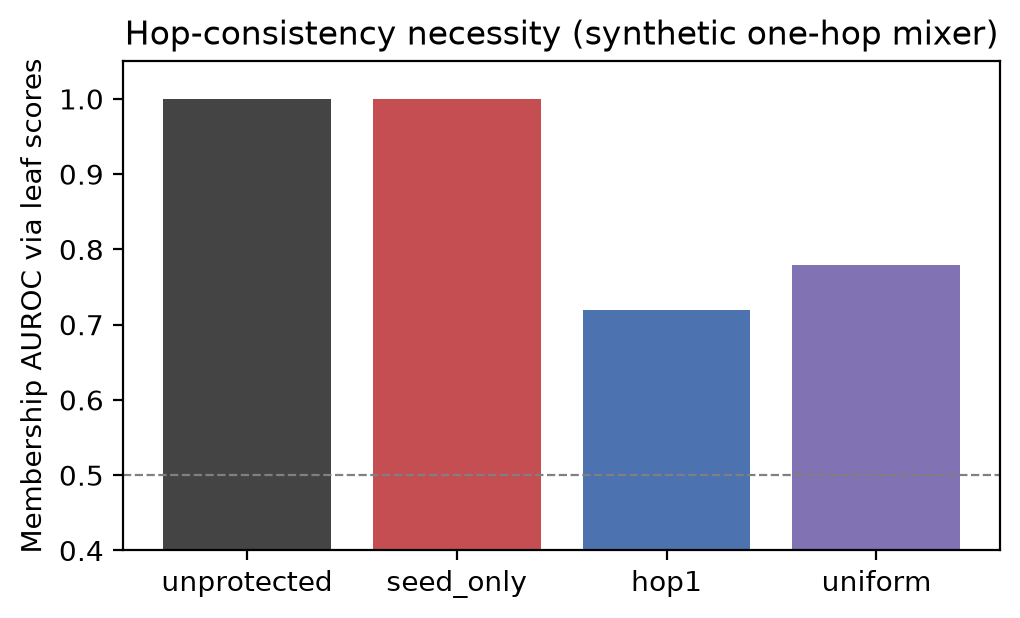
\includegraphics[width=0.49\linewidth]{fig_harp_hop_necessity.png}
\hfill

\includegraphics[width=0.49\linewidth]{fig_harp_cache_veracity.png}
\caption{Left: hop necessity (Prop.~\ref{thm:hop-necessary})---seed-only leaves leaf AUROC at $1.0$; hop-$1$ lowers it to ${\approx}0.72$. Right: score-cache hits under re-query traffic (Table~\ref{tab:cache}).}
\label{fig:hop-cache}
\end{figure}

\paragraph{Why ExactFrac matters (cache simulation).}
A Cora-sized synthetic API ($800$ clients $\times$ $25$ re-queries; exact-match score cache) makes veracity concrete (Fig.~\ref{fig:hop-cache}, right; Table~\ref{tab:cache}): fresh LBP hits $0\%$; HARP hits ${\approx}54\%$ from ExactFrac alone; $B{=}1$ freezes both, but only HARP keeps $c{=}0.60$ for consumers needing bit-identical softmax vectors.

\begin{table}[!t]
\caption{Score-cache simulation (Cora-sized; ExactFrac $c$ is by design).}
\label{tab:cache}
\centering
\scriptsize
\begin{tabular}{@{}lccc@{}}
\toprule
\textbf{Policy} & $\mathbf{c}$ & \textbf{Hit rate} & \textbf{Bit-exact re-query} \\
\midrule
None & $1.00$ & $0.865$ & $1.000$ \\
LBP fresh & $0.00$ & $0.000$ & $0.000$ \\
LBP $B{=}1$ & $0.00$ & $0.865$ & $1.000$ \\
HARP fresh & $0.60$ & $0.537$ & $0.563$ \\
HARP $B{=}1$ & $0.60$ & $0.865$ & $1.000$ \\
\bottomrule
\end{tabular}
\end{table}

\paragraph{Qualitative failure case (Chameleon).}
Population metrics hide mechanism.
Of $375$ protected train nodes (seed $42$), only $13$ (${\approx}3.5\%$) failed to shrink their train$-$test true-class confidence gap under HARP---overall mean gap falls $0.46\rightarrow 0.11$.
Manual inspection of those $13$ failures shows a recurring pattern: Lap$(\sigma{=}0.3)$ plus renormalization can \emph{increase} true-class confidence on some draws (e.g., node $177$: $0.78\rightarrow 1.00$; node $381$: $0.34\rightarrow 0.81$), concentrating mass on the true class by chance.
Peaky clean posteriors (conf$>0.9$) are also hard to flatten.
The takeaway for operators: HARP softens the mid-confidence mass that drives population LiRA, but a small overconfident/unlucky tail remains.
Raise Frac or $\sigma$ on that slice if canaries demand it; do not expect uniform-LBP-level erasure at ExactFrac${=}0.60$.

\paragraph{Adaptive LTE-aware queries.}
\label{sec:adaptive}
Table~\ref{tab:adaptive}: querying unprotected nodes, boundary cleans, or top-decile LTE seeds raises conf AUROC $0.513\rightarrow 0.638$--$0.651$ under locked HARP, while subset LiRA stays near population (${\approx}0.53$--$0.54$).
Population LiRA understates conf-MIA on the clean majority---log those canaries and raise Frac or $B$ if they drift.
Raising Frac to $0.60$ drops the top-decile LTE canary ($0.651\rightarrow 0.505$), but residual clean-slice conf AUROC stays elevated (${\approx}0.63$); pair Frac escalation with $B{=}1$.

\begin{table}[!t]
\caption{LTE-aware adaptive queries on Cora HARP (3 seeds).}
\label{tab:adaptive}
\centering
\scriptsize
\begin{tabular}{@{}lccc@{}}
\toprule
\textbf{Query set} & \textbf{Conf@0.4} & \textbf{Conf@0.6} & \textbf{LiRA@0.4} \\
\midrule
Population & 0.513 & 0.471 & 0.534 \\
Unprotected (clean) & 0.638 & 0.632 & 0.539 \\
Boundary (clean) & 0.626 & 0.634 & 0.535 \\
Top-decile LTE & 0.651 & 0.505 & 0.532 \\
\bottomrule
\end{tabular}
\end{table}

\paragraph{Inductive edge exclusion.}
\label{sec:inductive}
Dropping test-incident edges (Cora; 3 seeds) raises undefended LiRA to $0.631$ (TPR@1\% FPR $0.036$).
HARP recovers Acc $0.486\rightarrow 0.620$ vs.\ strong LBP at Frac${=}0.40$ (LiRA $0.569$; ECE $0.037$).
At Frac${=}0.60$, Acc falls to $0.549$ while LiRA improves to $0.559$---inductive audits may warrant a higher Frac on the same dial.

\subsection{When to spend: volume $\times$ structure}
Table~\ref{tab:audit}(a): undefended LiRA concentrates in small/mid heterophilic cells; Photo/PubMed/ogbn-arxiv sit near chance under matched shadows---audit first, then set Frac.
Table~\ref{tab:audit}(b) reports the honest shadow-count story on Cora for none / LBP / HARP.
Absolute LiRA rises with $n_{\mathrm{shadows}}$ for every defense~\cite{carlini2022membership}; Acc is invariant.
HARP does \emph{not} beat strong LBP on LiRA at large shadow counts (Cora $n_{\mathrm{sh}}{=}64$: LBP $0.561$ vs.\ HARP $0.677$)---expected when ExactFrac$=0$ is allowed.
What HARP keeps is (i)~strictly lower LiRA than undefended and (ii)~Acc recovery vs.\ strong LBP ($\Delta$Acc $+0.12$, invariant in $n_{\mathrm{sh}}$).
TPR@1\% FPR follows the same pattern.

\begin{table}[!t]
\caption{Audit controls (GraphSAGE; 3 seeds). $^\star$heterophilic. (b)~comparative shadow scaling (not HARP-only).}
\label{tab:audit}
\centering
\scriptsize
\begin{minipage}[t]{0.42\linewidth}
\centering
\textbf{(a) Undefended LiRA} ($n_{\mathrm{sh}}{=}4$)\\[0.2em]
\begin{tabular}{@{}lrrr@{}}
\toprule
\textbf{Dataset} & $\mathbf{n}$ & \textbf{Acc} & \textbf{LiRA} \\
\midrule
Chameleon$^\star$ & 2\,277 & 0.449 & 0.623 \\
Cora & 2\,708 & 0.879 & 0.568 \\
Actor$^\star$ & 7\,600 & 0.335 & 0.610 \\
Photo & 7\,650 & 0.825 & 0.500 \\
PubMed & 19\,717 & 0.876 & 0.505 \\
ogbn-arxiv & 169\,343 & 0.666 & 0.503 \\
\bottomrule
\end{tabular}
\end{minipage}\hfill
\begin{minipage}[t]{0.56\linewidth}
\centering
\textbf{(b) Cora shadow scaling (LiRA / TPR@1\%)}\\[0.2em]
\begin{tabular}{@{}lccc@{}}
\toprule
$\mathbf{n_{\mathrm{sh}}}$ & \textbf{none} & \textbf{LBP} & \textbf{HARP} \\
\midrule
4 & 0.568 / 0.033 & 0.517 / 0.022 & 0.534 / 0.014 \\
16 & 0.808 / 0.201 & 0.555 / 0.008 & 0.670 / 0.057 \\
64 & 0.847 / 0.265 & 0.561 / 0.008 & 0.677 / 0.075 \\
\bottomrule
\end{tabular}\\[0.4em]
{\scriptsize Acc invariant: none $0.879$, LBP $0.716$, HARP $0.836$. Chameleon mirrors the pattern (at $n_{\mathrm{sh}}{=}64$: none $0.965$, LBP $0.685$, HARP $0.811$; $\Delta$Acc vs.\ LBP $+0.061$).}
\end{minipage}
\end{table}

\subsection{Canaries and large-graph volume}
Table~\ref{tab:canary-ogbn}(a): HARP suppresses planted/top-decile confidence cues relative to none/LBP; population LiRA remains primary.
Table~\ref{tab:canary-ogbn}(b): on ogbn-arxiv (${\sim}169$k; NeighborLoader; gate off, warmup $3$)~\cite{hu2020ogb}, strong LBP drops Acc to $0.179$ $[0.175,0.184]$.
HARP recovers $0.599$ $[0.597,0.601]$ (paired $\Delta$Acc $+0.420$ $[0.414,0.425]$; 3 seeds) at Frac${=}0.40$.
Defense-aware LiRA stays near chance at both $n_{\mathrm{sh}}{=}2$ and $n_{\mathrm{sh}}{=}4$---a volume Acc-recovery result under an audit-null regime, not a claim that ogbn needs Frac${>}0$.
On ogbn-products (${\sim}2.4$M nodes)~\cite{hu2020ogb}, Table~\ref{tab:products} reports a systems probe on a $16$\,GB host plus a defense-aware LiRA audit on a BFS-induced $15$k-node subgraph ($829$k edges; $n_{\mathrm{sh}}{=}2$).
HARP recovers Acc $0.343\rightarrow 0.686$ vs.\ strong LBP while LiRA stays near chance.
Full-graph products LiRA exceeds host memory; the BFS subsample closes that gap without inventing a full-graph privacy claim.
The Big Data boundary is clear: release accounting and loader serving scale; full-graph shadow audits need more RAM or distributed training.

\begin{table}[!t]
\caption{ogbn-products: systems probe (full graph) and BFS-induced $15$k-node LiRA audit ($829$k edges; 3 seeds; $n_{\mathrm{sh}}{=}2$).}
\label{tab:products}
\centering
\scriptsize
\begin{tabular}{@{}lcccc@{}}
\toprule
\textbf{Setting} & $\mathbf{n}$ & \textbf{Acc} & \textbf{LiRA} & \textbf{Mass / RSS} \\
\midrule
Load graph & $2.45$M & --- & --- & RSS ${\approx}6.2$\,GB \\
Train none (subsample Acc) & $2.45$M & $0.695$ & --- & RSS ${\approx}7.4$\,GB \\
Strong LBP budget & $2.45$M & --- & --- & Mass ${\approx}7.3{\times}10^5$ \\
HARP budget (Frac${=}0.40$) & $2.45$M & --- & --- & Mass ${\approx}2.9{\times}10^5$ \\
\midrule
BFS-sub none & $15$k & $0.874$ & $0.506$ & --- \\
BFS-sub LBP $b{=}0.3$ & $15$k & $0.343$ & $0.500$ & --- \\
BFS-sub HARP & $15$k & $0.686$ & $0.503$ & --- \\
\bottomrule
\end{tabular}
\end{table}
If audit LiRA${\approx}0.5$, prefer Frac${=}0$; if LiRA$\gg 0.5$ or veracity requires ExactFrac$\ge c$, set Frac on val Acc (Frac${=}0.2$ maximizes Acc on Cora/Chameleon; Frac${=}0.4$ is the locked compliance default with $60\%$ exact responses).

\begin{table}[!t]
\caption{Canaries (left) and ogbn-arxiv volume (right; 3 seeds). LiRA shown for $n_{\mathrm{sh}}{=}2$ (primary) and $n_{\mathrm{sh}}{=}4$ (stress).}
\label{tab:canary-ogbn}
\centering
\begin{minipage}[t]{0.48\linewidth}
\centering
\footnotesize
\textbf{(a) Cora canaries}\\[0.3em]
\begin{tabular}{@{}lcccc@{}}
\toprule
\textbf{Def.} & \textbf{LiRA} & \textbf{Top} & \textbf{Plt.} & \textbf{ECE} \\
\midrule
none & 0.568 & 0.551 & 0.527 & 0.053 \\
LBP & 0.517 & 0.548 & 0.543 & 0.146 \\
HARP & 0.534 & 0.266 & 0.423 & 0.037 \\
\bottomrule
\end{tabular}
\end{minipage}\hfill
\begin{minipage}[t]{0.48\linewidth}
\centering
\footnotesize
\textbf{(b) ogbn-arxiv}\\[0.3em]
\begin{tabular}{@{}lcccc@{}}
\toprule
\textbf{Def.} & \textbf{Acc} & \textbf{LiRA$_2$} & \textbf{LiRA$_4$} & \textbf{Mass} \\
\midrule
none & 0.666 & 0.502 & 0.503 & --- \\
LBP & 0.179 & 0.498 & 0.501 & 50\,803 \\
HARP & 0.599 & 0.514 & 0.505 & 20\,322 \\
\bottomrule
\end{tabular}
\end{minipage}
\end{table}

\paragraph{Systems microbenchmarks.}
Cora setup ${\approx}41$\,ms; HARP release ${\approx}0.51$\,ms vs.\ LBP ${\approx}0.71$\,ms; products ${\approx}3.3{\times}10^3$ QPS at ${\approx}7.4$\,GB RSS.

\paragraph{Operator workflow.}
Audit with defense-aware LiRA; log Mass/Frac/ECE/unprot-conf.
If LiRA${\approx}0.5$, set Frac${=}0$; else select Frac on validation Acc (Table~\ref{tab:frac}), enforce session budget $B{=}1$ by default (Table~\ref{tab:session}), and use GAP when a legal $\varepsilon$ is required~\cite{sajadmanesh2023gap}.
On Cora/Chameleon, val Acc selection recovers the Acc-maximizing Frac in the grid (Frac${=}0.2$ matches the test oracle); LiRA or ExactFrac constraints instead pick a higher Frac on the same Pareto frontier.
Re-audit after model or graph updates.

\subsection{Protocol limitations}
Equal-mass and MemGuard can beat HARP on Acc--LiRA when ExactFrac$=0$ is allowed; selective masking raises LiRA; multi-query needs $B{=}1$ for a one-shot guarantee; adaptive conf AUROC remains elevated on residual clean nodes even at Frac${=}0.60$ (Table~\ref{tab:adaptive}); HARP is not DP; ogbn-products full LiRA needs more RAM/distributed shadows.

\section{Discussion}
\label{sec:discussion}

\subsection{What HARP is for}
HARP is for teams that serve GNN scores as a data product and need three things at once: usable accuracy, a clean majority of reproducible probabilities (ExactFrac$\ge c$), and an auditable noise budget.
It is \emph{not} a drop-in replacement for formal differential privacy: when a legal $\varepsilon$ is required, use training-time DP such as GAP~\cite{sajadmanesh2023gap,nasr2019comprehensive}.
Membership audits (LiRA) tell the operator whether Frac should be zero or positive; Acc and ECE tell them what the chosen Frac costs.
When LiRA${\approx}0.5$, the systems recommendation is Frac${=}0$.
When policy still mandates strong $\sigma$ \emph{or} ExactFrac$\ge c{>}0$, selective release is the feasible class; uniform LBP is not (Remark~\ref{rem:uniform-infeasible}).

\paragraph{How to score this paper.}
On Big Data criteria (ExactFrac as a Veracity SLA, Mass/Frac telemetry, Acc recovery vs.\ strong LBP, scale audits), judge HARP as a systems release policy.
On PETS/CCS criteria (new $(\varepsilon,\delta)$ mechanisms or Acc--LiRA dominance under ExactFrac$=0$), this paper declines; those problems are answered by GAP or uniform noise.

\subsection{Impact for Big Data graph APIs}
Hop-consistent release sets are the analogue of topology-aware row budgets; Mass/Frac give spend telemetry.
ExactFrac enables score-cache hits that uniform noise cannot (Table~\ref{tab:cache}); heterophilic graphs recover Acc vs.\ $b{=}0.3$; audit-null large graphs argue against blanket noise.

\subsection{Threats to validity}
Cora fairness/Frac: five seeds with paired CIs; other cells: three seeds.
Mass/Frac are spend metrics, not $(\varepsilon,\delta)$; ExactFrac/ECE measure fidelity, not per-node hardness.
Products subsample LiRA and ogbn-arxiv $n_{\mathrm{sh}}{=}4$ extend scale audits without claiming full-graph products privacy.

\subsection{Relation to formal differential privacy}
Prop.~\ref{thm:local-eps}: finite local $\varepsilon$ on the protected minority, $\varepsilon{=}\infty$ on the clean majority---hence infinite global $\varepsilon$ whenever ExactFrac$>0$.
That incompatibility is the constrained-release tradeoff.
Use GAP for regulatory DP; use HARP when ExactFrac$\ge c$ matters.

\subsection{What we do not claim}
HARP is not a stronger membership defense than uniform noise; does not dominate equal-mass/MemGuard when ExactFrac$=0$; hop $k$ is not a monotone LiRA lever; multi-query without $B$ erodes the one-shot defense; clean-slice conf-MIA stays elevated unless Frac or $B$ rises (Table~\ref{tab:adaptive}).

\subsection{Future work}
Adaptive Frac from streaming audits, co-optimizing formal $\varepsilon$ with Mass~\cite{mironov2017rdp,jayaraman2019evaluating}, federated hop-respecting APIs, and distributed LiRA at products/papers100M scale.

\section{Conclusion}
\label{sec:conclusion}
We proposed HARP, a selective release framework for GNN prediction APIs under constrained score release: maximize accuracy subject to a membership audit and a minimum exact-response fraction.
HARP is not a stronger membership defense than uniform noise; it is the feasible mechanism under ExactFrac$\ge c{>}0$, with hop-consistent allocation (Prop.~\ref{thm:hop-necessary}), selective local-$\varepsilon$ accounting (Prop.~\ref{thm:local-eps}), and Acc/calibration recovery versus strong LBP---including a quantified cache-hit benefit from the clean majority.
On six benchmarks plus OGB scale-ups with defense-aware LiRA, membership audits guide \emph{when} to spend budget; Frac and $B$ are the operator dials.
Use training-time DP when a legal global $\varepsilon$ is required.

\paragraph{Reproducibility.}
Code (\texttt{defenses/harp.py}, \texttt{defenses/memguard.py}, \texttt{run\_harp\_eval.py}), locked configs, and frozen CSVs accompany the submission artifact at \url{https://github.com/krishharma/privacy-gnn}.
Runs used Darwin arm64 CPU; LiRA $n_{\mathrm{shadows}}{=}4$ primary ($16$/$64$ comparative sweeps on Cora/Chameleon).

\balance
\begin{thebibliography}{00}
\bibitem{shokri2017membership} R. Shokri, M. Stronati, C. Song, and V. Shmatikov, ``Membership inference attacks against machine learning models,'' in \emph{Proc. IEEE Symp. Security Privacy (S\&P)}, 2017, pp. 3--18.
\bibitem{salem2019mlleaks} A. Salem, Y. Zhang, M. Humbert, P. Berrang, M. Fritz, and M. Backes, ``ML-Leaks: Model and data independent membership inference attacks and defenses on machine learning models,'' in \emph{Proc. NDSS}, 2019.
\bibitem{yeom2018privacy} S. Yeom, I. Giacomelli, M. Fredrikson, and S. Jha, ``Privacy risk in machine learning: Analyzing the connection to overfitting,'' in \emph{Proc. IEEE CSF}, 2018, pp. 268--282.
\bibitem{carlini2022membership} N. Carlini, S. Chien, M. Nasr, A. Song, T. Terzis, and F. Tramer, ``Membership inference attacks from first principles,'' in \emph{Proc. IEEE S\&P}, 2022, pp. 1897--1914.
\bibitem{olatunji2021mia} I. E. Olatunji, W. Nejdl, and M. Khosla, ``Membership inference attack on graph neural networks,'' arXiv:2101.06570, 2021.
\bibitem{jia2019memguard} J. Jia, A. Salem, M. Backes, Y. Zhang, and N. Z. Gong, ``MemGuard: Defending against black-box membership inference attacks via adversarial examples,'' in \emph{Proc. ACM CCS}, 2019, pp. 259--274.
\bibitem{wu2021mia} Y. Wu, D. Li, B. Chen, and L. Shen, ``Adapting membership inference attacks to GNN for graph classification,'' in \emph{Proc. IEEE ICDM}, 2021, pp. 1429--1434.
\bibitem{survey2023gnnprivacy} Y. Zhang, Y. Zhao, Z. Li, X. Cheng, Y. Wang, O. Kotevska, P. S. Yu, and T. Derr, ``A survey on privacy in graph neural networks: Attacks, preservation, and applications,'' arXiv:2308.16375, 2023.
\bibitem{kipf2017gcn} T. N. Kipf and M. Welling, ``Semi-supervised classification with graph convolutional networks,'' in \emph{Proc. ICLR}, 2017.
\bibitem{hamilton2017graphsage} W. L. Hamilton, R. Ying, and J. Leskovec, ``Inductive representation learning on large graphs,'' in \emph{Proc. NeurIPS}, 2017.
\bibitem{rong2020dropedge} Y. Rong, W. Huang, T. Xu, and J. Huang, ``DropEdge: Towards deep graph convolutional networks on node classification,'' in \emph{Proc. ICLR}, 2020.
\bibitem{choquette2021labelonly} C. A. Choquette-Choo, F. Tramer, N. Carlini, and N. Papernot, ``Label-only membership inference attacks,'' in \emph{Proc. ICML}, 2021, pp. 1964--1974.
\bibitem{sajadmanesh2023gap} S. Sajadmanesh et al., ``GAP: Differentially private graph neural networks with aggregation perturbation,'' in \emph{Proc. USENIX Security}, 2023, pp. 3229--3246.
\bibitem{abadi2016deepdp} M. Abadi et al., ``Deep learning with differential privacy,'' in \emph{Proc. ACM CCS}, 2016, pp. 308--318.
\bibitem{nasr2018advreg} M. Nasr, R. Shokri, and A. Houmansadr, ``Machine learning with membership privacy using adversarial regularization,'' in \emph{Proc. ACM CCS}, 2018, pp. 634--646.
\bibitem{nasr2019comprehensive} M. Nasr, R. Shokri, and A. Houmansadr, ``Comprehensive privacy analysis of deep learning,'' in \emph{Proc. IEEE S\&P}, 2019, pp. 739--753.
\bibitem{guo2017calibration} C. Guo, G. Pleiss, Y. Sun, and K. Q. Weinberger, ``On calibration of modern neural networks,'' in \emph{Proc. ICML}, 2017, pp. 1321--1330.
\bibitem{zhu2020beyondhomophily} J. Zhu et al., ``Beyond homophily in graph neural networks: Current limitations and effective designs,'' in \emph{Proc. NeurIPS}, 2020.
\bibitem{pei2020geomgcn} H. Pei, B. Wei, K. C.-C. Chang, Y. Lei, and B. Yang, ``Geom-GCN: Geometric graph convolutional networks,'' in \emph{Proc. ICLR}, 2020.
\bibitem{lim2021linkx} D. Lim, F. Hohne, X. Li, S. L. Huang, V. Gupta, O. Bhalerao, and S. N. Lim, ``Large scale learning on non-homophilous graphs: New benchmarks and strong simple methods,'' in \emph{Proc. NeurIPS}, 2021.
\bibitem{gtd2024} P. Niu, C. Pan, S. Chen, and O. Milenkovi\'c, ``Graph Transductive Defense: a Two-Stage Defense for Graph Membership Inference Attacks,'' arXiv:2406.07917, 2024.
\bibitem{maskarmor2024} C. Chen, X. Zhang, H. Qiu, J. Lou, Z. Liu, and X. Chen, ``MaskArmor: Confidence masking-based defense mechanism for GNN against MIA,'' \emph{Information Sciences}, vol. 669, 2024.
\bibitem{dps2025} M.~A.~P.~Chamikara et al., ``Can diffusion-based posterior smoothing secure GNNs from membership inference attacks?'' in \emph{Proc. AICCSA}, 2025.
\bibitem{duddu2020quantifying} V. Duddu, A. Boutet, and V. Shejwalkar, ``Quantifying privacy leakage in graph embedding,'' in \emph{Proc. WSDM}, 2020, pp. 76--84.
\bibitem{fredrikson2015modelinversion} M. Fredrikson, S. Jha, and T. Ristenpart, ``Model inversion attacks that exploit confidence information,'' in \emph{Proc. ACM CCS}, 2015, pp. 1322--1333.
\bibitem{tramer2016stealing} F. Tram\`er et al., ``Stealing machine learning models via prediction APIs,'' in \emph{Proc. USENIX Security}, 2016, pp. 601--618.
\bibitem{dwork2006dp} C. Dwork, ``Differential privacy,'' in \emph{Proc. ICALP}, 2006, pp. 1--12.
\bibitem{hu2020ogb} W. Hu et al., ``Open graph benchmark: Datasets for machine learning on graphs,'' in \emph{Proc. NeurIPS}, 2020.
\bibitem{velickovic2018gat} P. Veli\v{c}kovi\'c et al., ``Graph attention networks,'' in \emph{Proc. ICLR}, 2018.
\bibitem{xu2019gin} K. Xu, W. Hu, J. Leskovec, and S. Jegelka, ``How powerful are graph neural networks?'' in \emph{Proc. ICLR}, 2019.
\bibitem{mironov2017rdp} I. Mironov, ``R\'enyi differential privacy,'' in \emph{Proc. IEEE CSF}, 2017, pp. 263--275.
\bibitem{jayaraman2019evaluating} B. Jayaraman and D. Evans, ``Evaluating differentially private machine learning in practice,'' in \emph{Proc. USENIX Security}, 2019, pp. 1895--1912.
\bibitem{song2017memorization} C. Song, T. Ristenpart, and V. Shmatikov, ``Machine learning models that remember too much,'' in \emph{Proc. ACM CCS}, 2017, pp. 587--601.
\bibitem{niculescu2005predicting} A. Niculescu-Mizil and R. Caruana, ``Predicting good probabilities with supervised learning,'' in \emph{Proc. ICML}, 2005, pp. 625--632.
\bibitem{gps2024} Y. Jiang et al., ``Unveiling privacy vulnerabilities: Investigating the role of structure in graph data,'' in \emph{Proc. ACM KDD}, 2024. (GPS: structure$\to$attribute leakage; GHRatio; learnable edge sampling.)
\bibitem{napgnn2023} Q. Yuan et al., ``Node-Aware Differentially Private Graph Neural Networks for Graph Representation Learning,'' arXiv:2308.04943, 2023.
\bibitem{aerni2024misleading} M. Aerni, J. Zhang, and F. Tram\`er, ``Evaluations of machine learning privacy defenses are misleading,'' in \emph{Proc. ACM CCS}, 2024.
\bibitem{he2021nodemia} X. He, R. Wen, Y. Wu, M. Backes, Y. Shen, and Y. Zhang, ``Node-level membership inference attacks against graph neural networks,'' arXiv:2102.05429, 2021.
\bibitem{khosla2026structure} M. Khosla, ``Impact of graph structure on membership-inference risk for graph neural networks,'' \emph{Proc. Priv. Enhancing Technol. (PoPETs)}, 2026.
\end{thebibliography}

\end{document}
